\documentclass{beamer}
\usetheme{metropolis}           % Use metropolis theme
\usefonttheme{professionalfonts}
\newtheorem{remark}{Remark}
\newcommand\textred[1]{{\color{red}#1}}
\newcommand\N{{\cal N}}
\renewcommand\M{{\cal M}}
\newcommand\vs{{\mathrm{v.s.}}}
\newcommand\Var{{\mathrm{Var}}}
\newcommand\BSS{{\mathrm{BSS}}}
\newcommand\WSS{{\mathrm{WSS}}}
\newcommand\TSS{{\mathrm{TSS}}}

\newcommand\eqskip{12pt}

\usepackage{listings}
\lstset{language=R,keywordstyle={\bfseries \color{blue}}}
\usepackage{xparse}
\title{Tutorial 11 for STAT 3004\\Final Review}

\date{\today}
\author{WANG, Lijun}
\institute{Department of Statistics, CUHK}

\usepackage{longtable}
\begin{document}
\maketitle

\section{Quick Review}

\begin{frame}{Standard tests}
\vspace{-8pt}
\begin{figure}
\centering
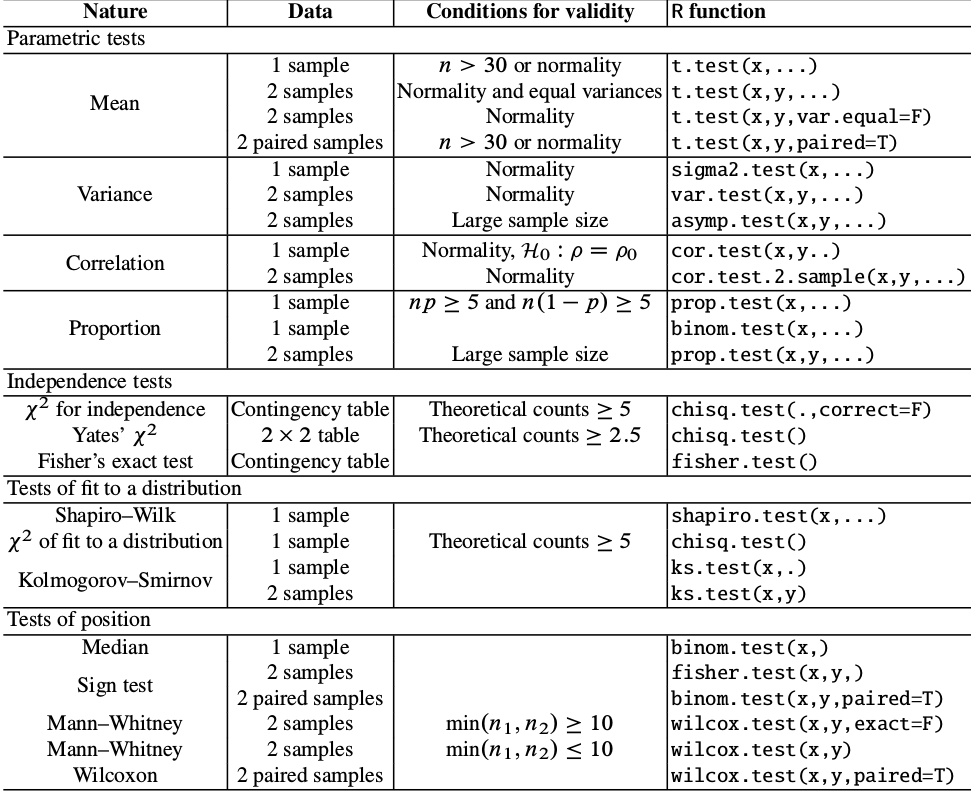
\includegraphics[width=0.95\textwidth]{standard-tests.png}
\end{figure}
\end{frame}

\section{Examples}

\begin{frame}{Cow study}
The quantity of bacteria per $\text{cm}^3$ of milk from eight different cows is estimated after milking and 24h later. We wish to test whether the quantity of bacteria significantly increases with time.
\begin{figure}
\centering
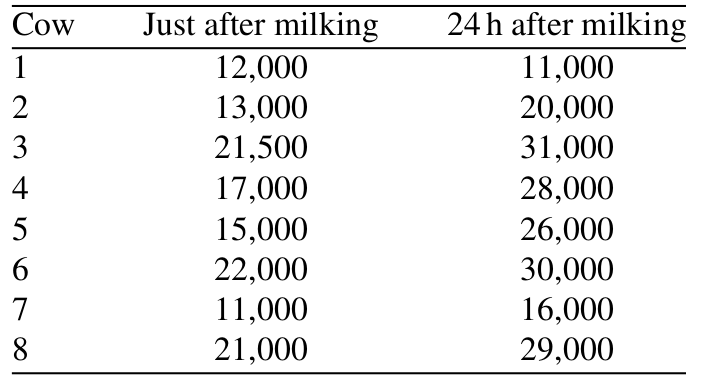
\includegraphics[width=0.6\textwidth]{cow-study.png}
\end{figure}
\begin{itemize}
\item Answer the question under the assumption of normality of the data.
\item Answer the question using a sign test.
\item Answer the question using a Wilcoxon's signed rank test.
\end{itemize}
\end{frame}

\begin{frame}{Number of patients in the emergency ward}
To study the variation of the number of emergency cases in a hospital, the number of patients was counted for the months of June, July and August. The results are
\begin{figure}
\centering
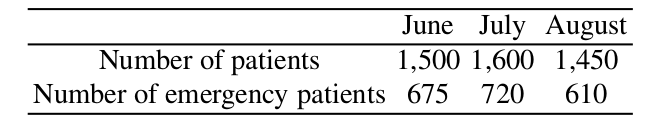
\includegraphics[width=0.95\textwidth]{num-patients.png}
\end{figure}
Can we conclude that the proportion of emergency cases is the same every month?

\end{frame}

\begin{frame}{Cell phone and driving reaction time}
Let's assume that you know from past experience that reaction time has a standard deviation of $1.25$ seconds. Also suppose that a $1$-second difference in reaction time is considered an important difference. You want to conduct a two-sided significance test at $5\%$ level with $90\%$ power to detect such a difference if it exists. How many participants will you need in your study?

To design such experiment, what else do you need?
\end{frame}

\begin{frame}
  \Huge{Gook luck!}
  \end{frame}
\end{document}